Nous appellerons ici \emph{réseau de choquet} un réseau de neurones ayant une architecture
adaptée a la regression d'une intégrale de choquet.
Comme vus precedement (\ref{subsec:intégrales-de-choquet}),
une fonction de choquet a une architecture complexe.
Voici l'intégrale de choquet entierement dévelopée pour un vecteur d'entrée taille $3$:
\begin{align*}
    C&\ =
    \color{red}
    w_1 \times x_1 + w_2 \times x_2 + w_3 \times x_3 \\
    \color{black}
    & +
    \color{blue}
    w_{m1} \times \min(x_1, x_2) + w_{m2} \times \min(x_1, x_3) + w_{m3} \times \min(x_2, x_3) \\
    \color{black}
    & +
    \color{green}
    w_{M1} \times \max(x_1, x_2) + w_{M2} \times \max(x_1, x_3) + w_{M3} \times \max(x_2, x_3)
\end{align*}
Voici l'architecture d'un réseau de choquet entierement générée par un réseau de neurones :

\begin{figure}[H]
    \center
    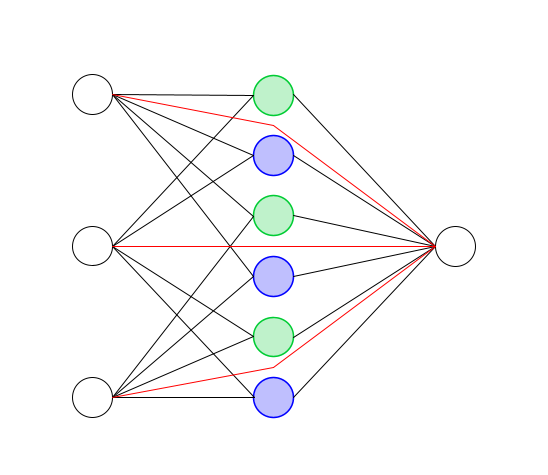
\includegraphics[height=\moyen]{pict/chnet1}
	\caption{Architecture d'un réseau de choquet}
	\label{fig:chnet1}
    \begin{center}
        \textit{
        En bleu, des neurone appliquant $\min(X)$, en vert $\max(X)$.
        }
    \end{center}
\end{figure}
\vspace{-12pt}
On peut voir que trois problemes non triviaux se posent :
\begin{itemize}
    \item Les neurones collorées n'appliquent pas une fonction simple.
    \item Les neurones ne sont pas reliés de manière simple (\textit{cf.}\ \ref{subsec:réseau-de-neurones}).
    \item Certains neurones passent des informations en sautant une couche de neurones.
\end{itemize}
Une autre piste à alors été envisagée :
Créer un réseau simple comme dans la figure suivante :
\begin{figure}[H]
    \center
    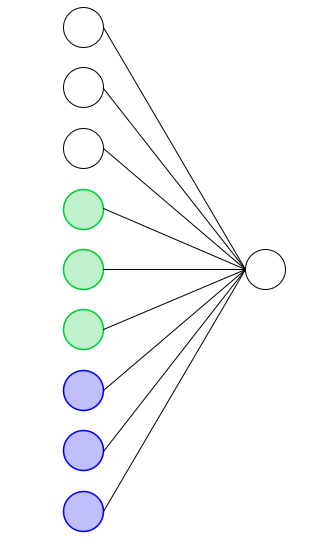
\includegraphics[height=\petit]{pict/net3.png}
	\caption{Réseau alternatif}
	\label{fig:net3}
\end{figure}
\vspace{-12pt}
Ici, aucuns neurone n'a de fonction spécifique, ceux de gauche sont les entrées
et celui de droite fait le produit scalaire avec un vecteur poid.
Ce réseau est bien plus simple à générer : c'est un réseau \emph{Dense} de taille $9$ en entrée.
Et plus généralement $n^2$ pour un vecteur de taille $n$.


\rbox{Démonstation :}
{
Prenons un vecteur de taille $n$,
Le but est d'énumerer le nombre de neurones utiles a la formule (\ref{eq:choquet}).
Le resultat est le suivant :
\begin{equation}
    n + \dbinom{n}{2} + \dbinom{n}{2} = n + 2 \times \frac{n(n-1)}{2} = n^2
\end{equation}
}

Il faut alors créer une base de donnée d'aprentissage à partir de chaqu'unes des fonctions d'utilitées
ce qui se fait tout simplement de la manière suivante :
\begin{lstlisting}[Language=Python]
def two_by_two(vector: iter, func: callable) -> np.array:
    out = np.array([])
    length = len(vector)
    for i in range(length):
        for j in range(i + 1, length):
            out = np.append(out, func(vector[[i, j]]))
    return out

Xs = np.concatenate((X, two_by_two(X, min), two_by_two(X, max)))
\end{lstlisting}
Lors de la descente de gradient, le réseau traite les poids indiférement, pour les récupérer,
il sufit de prendre les $n$ premiers pour $W$,
les $\frac{n(n-1)}{2}$ suivant pour $W_{\min}$
et les $\frac{n(n-1)}{2}$ derniers pour $W_{\max}$.